
\chapter{Présentation}
\label{chapter:poodlePres}

L'attaque Poodle (Padding Oracle On Downgraded Legacy Encryption)

a été découverte par Bodo Möller, Thai Duong et 
Krzysztof Kotowicz\cite{article:ssl-poodle} en septembre 2014.\\

Cette attaque se base sur une faiblesse de SSLv3.
Elle fonctionne pourtant sur les dernières versions de TLS.
Pour maintenir la compatibilité avec tout les clients, un
serveur TLS peut rétrograder en version SSLv3.\\

C'est une attaque de typer Man-In-The-Middle (l'homme du milieu).
L'attaquant peut utiliser un site malveillant qui injecte un
code javascript sur le client pour le faire générer des requêtes
sur le serveur cible. Il peut alors forcer l'utilisation de 
SSLv3, même si le client et le serveur utilisent TLS.\\

L'objectif de l'attaque est de voler le cookie de session 
du client. Pour cela, comme BEAST, l'attaquant force 
l'utilisation du mode CBC. Elle utilise le \emph{padding oracle attack }

\chapter{Padding Oracle Attack}
\label{chapter:POA}

Cette attaque a pour objectif de retrouver le clair d'un bloc chiffré 
avec le mode CBC. Elle s'appuie sur le fait que le dernier bloc chiffré
contient du padding. De plus le dernier octet de padding corespond à la
taille du padding.\\

L'oracle  déchiffre le clair et vérifie que la taille du padding est correcte. 
Il renvoie une erreur en cas de taille erronée.\\

Supposons maintenant que l'attaquant posséde un chiffré composé de 4 blocs :
$C1||C2||C3||C4$. Le bloc $C4$ contient un padding de taille $x$ connu par l'attaquant.
il souhaite connaitre le contenu de $C2$ et quand il interoge l'oracle, celui-ci lui dit
si la taille est correcte ou non.\\
L'attaquant peut envoyer une version contrefaites du chiffré comme suit :
$C1||C2||C3'||C4'$.\\
\begin{itemize}
\item le bloc $C4'=C2$
\item le bloc $C3'= C3$ dont le dernier octet est modifié
\end{itemize}
Soit $Pn$ le déchiffrement de $Cn$ par l'oracle et D() et E() les algorithmes
de déchiffement et de chiffrement. 
Le bloc qui nous intérésse est $P4'$.
\[P4' = D(C2) + C3'\]
or $C2 = E(P2 + C1)$ d'où

\[\Longleftrightarrow P4' = D(E(P2 + C1)) + C3'\]
\[\Longleftrightarrow P4' = P2 + C1 + C3'\]
\begin{itemize}
\item $C1$ et $C3'$ sont connus
\item $P2$ est le clair recherché
\item $P4'$ est inconnu mais l'oracle nous dit si le dernier octet égale à $x$.
\end{itemize}
Soit k la taille des blocs et Pn[i] le iéme octet du bloc n.

\[P4'[k] = P2[k] + C1[k] + C3'[k]\] si $P4'[k] = x$ alors
\[\Longleftrightarrow x = P2[k] + C1[k] + C3'[k]\]
\[\Longleftrightarrow P2[k] = x + C1[k] + C3'[k]\]

Ce qui donne une equation a une seule inconnu donc l'attaquant a trouvé $P2[k]$.
Pour avoir $P4' = x$, il suffit de faire varier la valeur de $C3'[k]$. Il est donc
possible de trouver le dernier octet de $P2$ en maximum de 256 essais.\\

Pour trouver les autres octets, l'attaquant prend $P4'[k] = P2[i]$ où $i \in [1,k]$.
Avec cette méthode il est possible de retrouver tout le contenu d'un chiffré à
l'exeption du premier bloc (sauf si l'IV est connu).

\chapter{Mise en place de l'attaque}
\label{chapter:Poodleattack}

\section{Packet SSL}

Le Format des paquets SSL est le suivant : 
\begin{center}
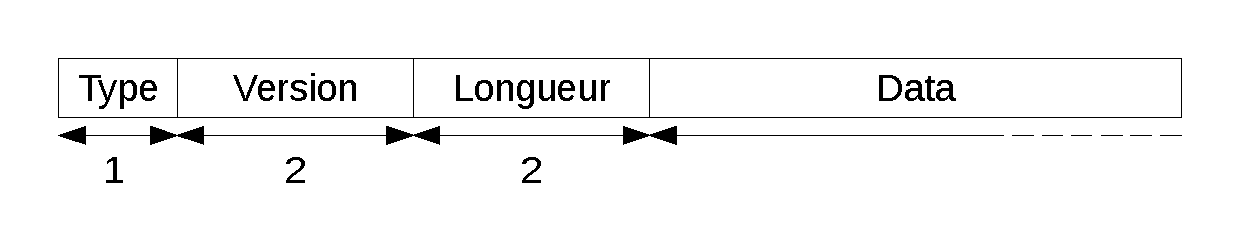
\includegraphics[scale=0.5]{schemaSSL.pdf}
\end{center}

Type :
\begin{itemize}
\item 0x16 : Handshake
\item 0x14 : Change Cypher Spec
\item 0x15 : Alert
\item 0x17 Application Data
\end{itemize}

Version :
\begin{itemize}
\item 0x3000 : SSLv3
\item 0x30xy : TLSvx.y
\end{itemize}

Les données sont chiffrées et leurs tailles est indiquées par
la longueur.




